\chapter{Motivação e visão geral do trabalho}
\label{chapter:intro}

O atual cenário de desenvolvimento tecnológico encontra-se no meio de uma quarta revolução industrial. Nunca se produziram tantos dados e se utilizaram redes como a própria internet para propaga-los. É de se esperar que tanto diferentes mercados demandem inovações para o compartilhamento desses dados em tempo real ou próximo a isso.

A Internet das Coisas é a rede que permite a conexão e compartilhamento de dados  de dispositivos físicos. Ela é derivada de métodos de comunicação entre máquinas e telemetria. Pode ser dissecada em três camadas de aquisição, comunicação e aplicação  podendo ser implementada utilizando diversos protocolos de comunicação, dependendo da tecnologia disponível. É importante que sistemas IoT sejam projetados de forma a atender a aplicação eficientemente, porém tal tarefa não é fácil nem simples. O trabalho propõe um sistema que permite facilitar tal tarefa.

Este projeto propõe uma interface para comunicação entre as diferentes tecnologias e protocolos de aplicação em redes, de forma que o desenvolvedor só se preocupe em  implementar e configurar uma interface para mapear a melhor opção de ferramentas para a aplicação. O projeto lida com protocolos baseados sobre o TCP/IP, uma unanimidade em redes conectadas a internet. Ele oferece uma API para aquisição, transmissão, recepção e armazenamento de dados telemétricos. O foco está no protocolo de aplicação MQTT (\textit{Message Queuing Telemetry Transport}) \cite{mqtt}, um protocolo que opera sobre o TCP/IP, leve e extremamente utilizado para compartilhamento  de dados telemétricos e de mensagens. Podendo se estender para outras protocolos de aplicações de escopo fechado.

\section{Internet das Coisas}
\label{section:iot}

"A Internet das Coisas tem o potencial de mudar o mundo. Assim como a Internet fez. Talvez até mais" \cite{ashton:iot}. Uma tradução livre de Rampim \cite{Rampim:iot} da frase de Kevin Ashton, cofundandor do Auto-ID Center, em 1999. Apesar de ser um nome feito somente para chamar atenção, foi a primeira citação da expressão Internet das Coisas.

Dentre as áreas da Indústria 4.0, encontra-se a internet das coisas ou IoT, responsável por estruturar as aplicações de aquisição, transmissão e armazenamento. Não é uma surpresa que a Internet das Coisas envolva áreas como eletrônica, computação e telecomunicações em um pacote só. De fato as camadas de IoT são mundos diferentes interligados para um propósito: transmitir dados sobre um dispositivo e/ou para um dispositivo em tempo real. Segundo a Cisco IBSG, Cisco Internet Business Solutions Group \cite{cisco:ibsg}, há mais objetos conectados que pessoas no mundo.

Pode-se definir IoT como a estrutura que comunica dispositivos em rede, permitindo a transmissão de dados sobre eles em tempo real. Essa estrutura permite a troca de informações sobre um dispositivo: seu estado, seu desempenho, suas condições físicas e do ambiente ao seu redor. Mas, para que este ciclo esteja completo são necessárias camadas que desempenham tarefas específicas, para que o dado chegue a quem ou a o que o está esperando.

\section{Visão geral de uma aplicação IoT}
\label{section:overview}

Na \ref{fig:1.1.0/iot_app}, temos uma rede de N sensores que enviam dados telemétricos e M atuadores que recebem ordens para executar uma função, todos estão em rede e podem receber e enviar informação em tempo real. O servidor, que pode ser um Broker como será descrito adiante nesse trabalho, encaminha os dados (ou mensagens) para o banco de dados. O Banco é utilizado para análise dos dados, o controlador por sua vez envia as mensagens de decisões baseada na análise de dados a serem transmitidas para os atuadores.

\begin{figure}[h!]
\centering
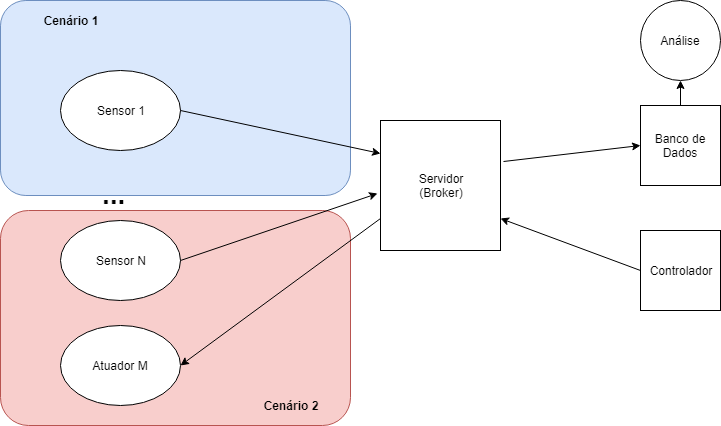
\includegraphics[width=10cm]{./02_Capitulos/02_Cap1/figures/iot_app}
\caption{Um exemplo de aplicação IoT que percorre os problemas a solucionar}
\label{fig:1.1.0/iot_app}
\end{figure}

O sensor 1 está imerso em um ambiente com as próprias características físicas e de rede, na verdade, cada sensor está imerso num cenário, que pode variar  de uma rede com poucos sensores a rede com grande fluxo de dados, sujeita a congestionamento. Assim, é fundamental que o  sistema se ajuste-se aos diferentes cenários.

Este trabalho visa implementar um sistema que utiliza o protocolo de aplicação MQTT, para transmissão de dados em tempo real entre dispositivos). O sistema contempla também persistência de dados utilizando banco de dados MongoDB e criará canais de dados (Data Streams), cuja função será adaptar a transmissão dos dados aos cenários onde apresentam limitações na conexão, seja por problemas de infraestrutura ou congestionamento na rede.

\begin{figure}[h!]
\centering
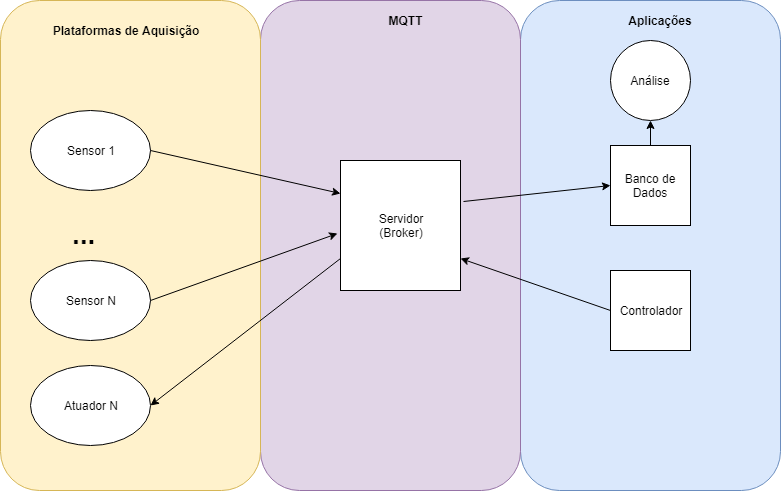
\includegraphics[width=10cm]{./02_Capitulos/02_Cap1/figures/iot_app-layers}
\caption{Diagrama de um exemplo de aplicação IoT dividida em blocos, cada um exercendo uma função em uma aplicação IoT}
\label{fig:1.1.0/iot_app-layers}
\end{figure}


Cada bloco da figura acima é responsável por uma tarefa no sistema IoT, da aquisição de dados a persistência destes, conforme ilustrados na \ref{fig:1.1.0/iot_app-layers}. Para entender melhor cada tarefa, será descrito o projeto e as implementações em cada bloco no sistema.

Inicialmente, os conceitos e ideias do projeto eram voltados a desenvolver uma interface na qual um desenvolvedor poderia implementar um sistema IoT de ponta a ponta utilizando APIs que direcionariam para um desses protocolos de tecnologias da seção \ref{section:tecnologias_iot}, porém as diferenças entre os protocolos e as camadas de base, fazem com que esta solução esteja mais distante. Então o foco voltou-se  para tecnologias que tenham base na pilha TCP/IP, por sua vasta implementação nas redes industriais e residências e na Internet.

\section{Interface para Protocolos de Aplicação}
\label{section:interface_iot}

Neste projeto será visto a implementação de uma interface entre o desenvolvedor e  o protocolo MQTT, implementando o conceito de canais de dados (Data Streams), como mostrado na \ref{fig:2.2.0/camada_abatracao}.  Algumas destas características podem ser destacadas:

\begin{itemize}

\item Multicast. Capaz de enviar mensagens a um ou mais dispositivos simultâneos;
\item Envio de mensagens em tempo real;

\end{itemize}


\begin{figure}[h!]
\centering
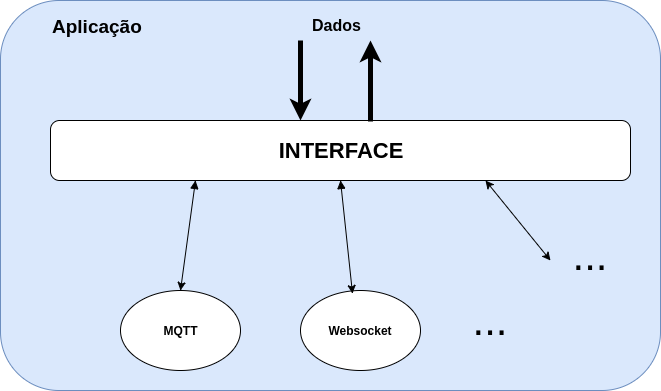
\includegraphics[width=12cm]{./02_Capitulos/02_Cap2/figures/camada_abstracao}
\caption{Interface de comunicação. A interface tem sua arquitetura que pode se comunicar com um ou mais protocolos de aplicação}
\label{fig:2.2.0/camada_abatracao}
\end{figure}

